% Modelo de Dissertação em Latex para o PPG em Engenharia Mecânica da UERJ
% Este modelo foi adaptado da versão disponibilizada no site da Engenharia Elétrica da UERJ
% http://www.pel.uerj.br/publico/Modelo_LaTeX_Dissertacao_UERJ.rar
% http://www.pel.uerj.br/defesas/
%
% Utilizei o WinEdt 6.0 com Miktex 2.9
%
% Para gerar o PDF usei a opção PDFTeXfy com o documento [masterthesis.tex] aberto e em foco.
%
% Não consegui usar as figuras em EPS como o modelo original. Usei PNG e JPG sem problemas.
%
% Felipe M. - 20/06/2012
%




\documentclass[a4paper,12pt,oneside,openany]{uerj}

\usepackage[english,brazil]{babel}
%\usepackage[latin1]{inputenc}
\usepackage[utf8]{inputenc}
\usepackage{enumerate}
\usepackage{cite}
\usepackage{epsf,epsfig,psfig}
\usepackage{pagina}
\usepackage{indentfirst}
\usepackage{theorem}
\usepackage{fancyhdr}
\usepackage{setspace}
\usepackage{boxedminipage}
\usepackage{float}
\usepackage{makeidx}
\usepackage{amsmath}
\usepackage[hidelinks]{hyperref}
\usepackage{comment}
\usepackage[alf]{abntex2cite}
\usepackage{textcomp} %usar registered symbol ®
\usepackage{enumitem}


\makeindex


\newtheorem{deff}{Definição}[section]
\numberwithin{equation}{chapter}

\theoremstyle{plain}

\bibliographystyle{abnt-num}



\begin{document}

\hypersetup{
    colorlinks,
    citecolor=black,
    filecolor=black,
    linkcolor=black,
    urlcolor=black,
    linktoc=all
}

\thispagestyle{empty}\begin{titlepage}
\begin{center}

	\vspace{-0.5cm}

  \begin{figure}[hbt!]
		\begin{flushleft}
		   
\includegraphics[width=2.25cm,height=2.91cm]{./01_Pre_textuais/logoUfpe_pb.png}
		\end{flushleft}
	\end{figure}
	\vspace{-4cm}

  \hspace{2cm}\large{\textbf{UNIVERSIDADE FEDERAL DE PERNAMBUCO}}\\
  \hspace{2cm}\large{Centro de Tecnologia e Geociências}\\
  \hspace{2cm}\large{Curso de Graduação em Eng. de Controle e Automação}\\

  \hspace{2cm}\large{}\\
  \hspace{2cm}\large{}\\
  \hspace{2cm}\large{}\\
  \hspace{2cm}\large{}\\

  \par
  \large{Ezequiel Filipe Correia Reis}

  \hspace{2cm}\large{}\\
  \hspace{2cm}\large{}\\
  \hspace{2cm}\large{}\\
  \hspace{2cm}\large{}\\


  \par
  \large\textbf{Título do Trabalho}


  \par\vfill
  Recife\\Dezembro de 2018

\end{center}
\end{titlepage}
\pagebreak\thispagestyle{empty}\begin{center}

Ezequiel Filipe Correia Reis

% \vfill
\vspace{2cm}

\textbf{Título do Trabalho}

\vspace{1.0cm}

\begin{figure}[hbt!]
\begin{center}

\includegraphics[width=15.72cm,height=16.2cm]{./01_Pre_textuais/logoUfpe_gnd}
\end{center}
\end{figure}

\vspace{-9cm}
\begin{flushright}
\parbox{8cm}{
\singlespacing{Monografia apresentada ao curso de\linebreak Engenharia de Controle e Automação, como requisito parcial para a obtenção do Título de Bacharel em Engenharia de Controle e Automação, Centro de Tecnologia e Geociências da Universidade Federal de Pernambuco}.
}
\end{flushright}

\vspace{4.0cm}

Orientador: Prof. Dr. Márcio Evaristo da Cruz Brito\\

\par\vfill
%\vspace{2cm}

Recife\\Dezembro de 2018

\end{center}
\pagebreak\thispagestyle{empty}% Depois de preparar seu trabalho, você deverá enviá-lo para a Biblioteca CTC/B para avaliação do formato e elaboração da Ficha catalográfica.
% Com a ficha pronta (fornecida pela Biblioteca), você poderá alterar este trecho do trabalho em definitivo.
%
% Para este processo, enviei a dissertação em PDF para o email: ctcb.uerj.bdtd@gmail.com (Tratei de todos os detlahes com a Sra. Márcia)
% Qualquer dúvida, veja os contatos da Biblioteca no site da Rede Sirius: http://www.rsirius.uerj.br/
% 


\begin{titlepage}
	\begin{center}
\vfill
\singlespacing
	\vspace*{95mm}
	{CATALOGAÇÃO NA FONTE\\ \vspace{1.5mm}
	UERJ\,/\,REDE SIRIUS\,/\,BIBLIOTECA CTC/B}\\
	\vspace{1.5mm}
	\begin{boxedminipage}{140mm}
	\begin{minipage}{5mm}
		\vspace{-84mm}
		S237
	\end{minipage}
	\hfill
	\raisebox{8.5mm}{
	\begin{minipage}[top]{115mm}
		\vspace*{5mm}

		Sobrenome, Nome do Autor\\
		\phantom{XX}Título\,/\,Nome completo do autor. -- 2012.\\
		\phantom{XX}105\,f.\\
		\phantom{XX}\\
		\phantom{XX}Orientadores: Nome completo do orientador1;\\
\hspace*{5mm}
Nome completo do orientador2\\
       		\phantom{XX}Dissertação(Mestrado) -- Universidade do Estado do Rio de Janeiro, Faculdade de Engenharia.\\
		\phantom{XX}\\
		\phantom{XX}Texto a ser informado pela biblioteca.
	\end{minipage}}
	\vspace*{5mm}
	\begin{flushright}
	 CDU~621:528.8
	\end{flushright}
    \vspace{1mm}
	\end{boxedminipage}\\
	\end{center}
%
	Autorizo, apenas para fins acadêmicos e científicos, a reprodução total ou parcial desta dissertação, desde que citada a fonte.\\
	\noindent
	\begin{tabular}{ccc}
	\phantom{XXXXXXXXXXXXXXXXXXXXXXXXXXXXXX}&	 \phantom{XX}	&	\phantom{XXXXXXXXXXXXXXXX}	\\
	\phantom{XXXXXXXXXXXXXXXXXXXXXXXXXXXXXX}&	 \phantom{XX}	&	\phantom{XXXXXXXXXXXXXXXX}	\\
	\cline{1-1}\cline{3-3}
	Assinatura &		&	Data
	\end{tabular}
\end{titlepage}   
\pagebreak\thispagestyle{empty}\addtocounter{page}{+1}
\begin{center}

Nome do Aluno

\vspace{1cm}

\textbf{Título do Trabalho}

\end{center}

\vspace{.4cm}

\begin{flushright}
\parbox{8cm}{
\singlespacing{Dissertação apresentada, como requisito\linebreak parcial para obtenção do título de Mestre em Ciências, ao Programa de Pós-Graduação em Engenharia Mecânica, da Universidade do Estado do Rio de Janeiro. Área de\linebreak concentração: Fenômenos de Transporte}.
}
\end{flushright}

\vspace{.6cm}


% insira abaixo a data de sua defesa
% Caso não tenha defendido ainda, deixe em branco

\noindent Aprovado em: 29 de Maio de 2012

\noindent Banca Examinadora:


%
%
% Os professores da UERJ DEVEM ser citados primeiro, independente de quem seja o orientador.
%
%



\vspace{.7cm}

\begin{flushright}
\parbox{12cm}{

\singlespacing

\hrulefill \\

\vspace{-.4cm}
Prof. Dr. Nome do Professor 1 (Orientador)
\newline
Instituto de Matemática e Estatística da UERJ
\vspace{.7cm}

\hrulefill \\

\vspace{-.4cm}
Prof. Dr. Nome do Professor 2
\newline
Faculdade de Engenharia da UERJ
\vspace{.7cm}

\hrulefill \\

\vspace{-.4cm}
Prof. Dr. Nome do Professor 3
\newline
Universidade Federal do Rio de Janeiro - UFRJ - COPPE
\vspace{.7cm}

\hrulefill \\

\vspace{-.4cm}
Prof. Dr. Nome do Professor 4
\newline
Instituto de Geociências da UFF
\vspace{.7cm}

\hrulefill \\

\vspace{-.4cm}
Prof. Dr. Nome do Professor 5
\newline
Universidade Federal do Rio de Janeiro - UFRJ - COPPE
\vspace{.7cm}

}
\end{flushright}
\vfill

\begin{center}
Rio de Janeiro\linebreak 2012
\end{center}
\pagebreak\thispagestyle{empty}\begin{center}
\textbf{DEDICATÓRIA}
\end{center}

$\!$\\

%\vspace{1cm}

Aqui entra sua dedicatória.
\pagebreak\thispagestyle{empty}\begin{center}
\textbf{AGRADECIMENTO}
\end{center}

$\!$\\

Aqui entra seu agradecimento.

É importante sempre lembrar do agradecimento à instituição que financiou sua bolsa, se for o caso...

Agradeço à FAPERJ pela bolsa de Mestrado concedida.
%\pagebreak\thispagestyle{empty}\input{./01_Pre_textuais/Epigrafe}    % não coloquei epígrafe no meu trabalho, mas fica aqui a chamada comentada.
\pagebreak\thispagestyle{empty}\begin{center}
\textbf{RESUMO}
\end{center}

%
% O resumo deve ser organizado em apenas um parágrafo mesmo.
% O número de folha é o número de páginas do PDF -2. Isto ocorre pois na versão final (capa dura) a capa é removida e as duas primeiras páginas são impressas em uma % folha apenas (frente e verso).
%

$\!$\\

\hspace{-1.3cm}\textbf{SOBRENOME}, Nome do autor. \textit{Título do Trabalho}. 105 f. Dissertação~(Mestrado em Engenharia Mecânica) - Faculdade de Engenharia, Universidade do Estado do Rio de Janeiro~(UERJ), Rio de Janeiro, 2012.

\vspace{.2cm}

Aqui entra o seu resumo organizado em um parágrafo apenas.

\vspace{1cm}

\hspace{-1.3cm}Palavras-chave: Palavra1, Palavra2, Palavra3, Palavra 4.
\pagebreak\thispagestyle{empty}\begin{center}
\textbf{ABSTRACT}
\end{center}

$\!$\\

% O resumo em inglês deve ser organizado em apenas um parágrafo mesmo.

Aqui entra seu resumo em inglês também organizado em apenas um parágrafo.

\vspace{1cm}

\hspace{-1.3cm}Keywords: Word1, Word2, Word3, Word4.

\fancypagestyle{plain}{
\fancyhf{} % clear all header and footer fields
\renewcommand{\headrulewidth}{0pt}
\renewcommand{\footrulewidth}{0pt}}
\pagestyle{plain}

\pagebreak

\def\listfigurename{LISTA DE FIGURAS}\listoffigures
\def\listtablename{LISTA DE TABELAS}\listoftables
%\newpage

\begin{center}
\textbf{LISTA DE SIGLAS}
\end{center}
$\!$\\

\begin{tabular}{lll}
3GPP & \hspace{1cm} & Third Generation Partnership Project \\
AGPS &  \hspace{1cm} & Assisted Global Positioning System \\
ANATEL &  \hspace{1cm} & Agência Nacional de Telecomunicações \\
ANN & \hspace{1cm} & Artificial Neural Network \\
AOA&  \hspace{1cm} &Angle of Arrival \\
AP&  \hspace{1cm} &Access Point \\
BCCH&  \hspace{1cm} &Broadcast Control Channel \\
\end{tabular}    % não coloquei LISTA DE SIGLAS no meu trabalho, mas fica aqui a chamada comentada.
\def\contentsname{SUMÁRIO}\tableofcontents

\fancypagestyle{plain}{
\fancyhf{} % clear all header and footer fields
\fancyhead[R]{\thepage}
\setlength{\voffset}{-1cm}
\setlength{\headsep}{1cm}
\renewcommand{\headrulewidth}{0pt}
\renewcommand{\footrulewidth}{0pt}}

\pagestyle{plain}

\pagebreak
\addcontentsline{toc}{chapter}{\hspace{1.7cm}\bfseries INTRODUÇÃO}
\noindent\textbf{INTRODUÇÃO}
$\!$\\

Aqui entra sua introdução!!


%\chapter{REVISÃO BIBLIOGRÁFICA}
\label{chapter:exemplo}
\section{\textbf{Sistemas Embarcados}}
\label{sec:SistemasEmbarcados}
\subsection{\textbf{Conceitos Preliminares}}
\label{subsec:sub01_Conceitos}

\subsection{\textbf{Definição de Sistemas Embarcados}}
\label{subsec:sub01_Definicao}
Um sistema embarcado pode ser definido, como um sistema computacional, interno a um dispositivo eletrônico, que executa, repetitivamente, uma única função, ou um pequeno conjunto de funções, de maneira que, frequentemente, a forma que estas tarefas são executadas não é percebida pelo seu usuário, assim como expõe \citeonline[p.~1]{Chatto2013}, mas sim os resultados da realização das mesmas. Já o termo “sistema embarcado” deriva do fato que estes sistemas são totalmente integrados e enclausurados pelos sistemas a que servem ou controlam, dessa forma, com este enclausuramento, tem-se como consequência que estes sistemas se tornam especializados em realizar tarefas específicas à operação do dispositivo que o contém, \cite[p.~554]{Springer2009}. Essa especialização é notada no software embarcado, também chamado de firmware, que se torna específico ao hardware utilizado, e o próprio hardware, que tem características que o diferem de um hardware de sistema de propósito geral. 

Com o objetivo de deixar mais claro o que essa falta de generalidade relacionada a funcionalidade de um sistema embarcado implica, \citeonline[p.~2]{Steve2003} complementa ao dizer que tais sistemas não são construídos de forma a serem programados pelo usuário final, não da forma que um sistema genérico possibilita, pois, o usuário final de um sistema embarcado não pode alterar a funcionalidade do sistema, seja adicionando, ou mesmo retirando, software. Observe, por exemplo, que um computador pessoal, um exemplo de sistema de propósito geral, pode funcionar como um processador de texto e, em um instante, começar a funcionar como um navegador web, observe ainda que, é permitido, ao usuário, adicionar diversas funcionalidades ao sistema, sem que o sistema tenha vindo configurado para execução da nova funcionalidade de fábrica. 

\subsection{\textbf{Características}}
\label{subsec:sub01_Caracteristicas}
Algumas características dos sistemas embarcados serão descritas a seguir, que é uma breve explanação sobre alguns pontos apresentados por \citeonline[p.~2-4]{Chatto2013}, importante notar que a exibição de todas estas características descritas não é obrigatória, porém, são muito comuns e importantes nestes sistemas, e, geralmente, alguma delas se sobressai, dependendo da finalidade do sistema em questão.

 A interação com o ambiente é uma característica presente na maioria dos sistemas embarcados, esta é feita por meio de sensores, que coletam dados do ambiente, e, ou, de atuadores, que atuam em alguns parâmetros do ambiente. Através da interação com o ambiente, os sistemas embarcados podem ser sistemas reativos, ou seja, possuir interação contínua e reagir a eventos do ambiente, onde o sistema pode, por exemplo, apresentar estados que transitam em resposta à ocorrência de eventos, ou reagir, com o objetivo de controlar algum tipo de variável do ambiente. Pode-se citar ainda, como uma característica, a mistura de componentes digitais e analógicos, que é inerente a interação com o ambiente. O ambiente, cuja natureza é predominantemente contínua. Portanto, frequentemente, a natureza digital dos computadores se mescla com a natureza analógica do ambiente para a implementação de um sistema embarcado.
 
A interface com o usuário, comumente, é mais simples que a encontrada em sistemas mais genéricos, composta por componentes que geralmente causam a ilusão ao usuário de falta de computação, como LEDs e botões.

A limitação do sistema, este que é restringido de diversos ângulos. Nota-se que, um sistema embarcado, pela sua própria natureza limitada, possui limitações de performance e de consumo de energia, que influenciam na escolha do dispositivo alvo. Como exemplo, o volume físico é uma limitação de projeto muito comum, dentre tantas outras limitações específicas de cada projeto, com sua relevância intrínseca ao projeto, como robustez a variação de temperatura, resistência a radiação, ou vibração mecânica. De fato, nenhum sistema é de todo livre de restrições, porém, nos sistemas embarcados, essas restrições são muito mais evidentes e são, em certos casos, consequência de requisitos do sistema.

A confiabilidade do sistema, já que, como um sistema embarcado tem a capacidade de funcionar autonomamente, estes são empregados em diversas atividades de natureza crítica, o que exige, frequentemente, disponibilidade e manutenibilidade do sistema e também segurança da informação processada pelo sistema. 

Relacionado à confiabilidade, está também a característica de processamento em tempo real, que se refere a exigência de resposta em um tempo fixo e finito de tempo de uma requisição. O não cumprimento desta exigência pode levar a consequências catastróficas em sistemas de tempo real. 

\subsection{\textbf{Elementos de um Sistema Embarcado}}
\label{subsec:sub01_Elementos}
Um sistema embarcado, geralmente, é um sistema microprocessado, isto significa que o mesmo, geralmente, se utiliza de uma unidade central para o processamento, o processador. Este processador pode ser implementado através de dispositivos de hardware programável, como um FPGA, ou se utilizar de um processador dedicado disponível no mercado, ou ainda, caso não se utilize um processador formal, um sistema embarcado poderia ser ainda implementado com a utilização de circuitos lógicos digitais, sem perca de sua condição de sistema embarcado. Porém, essas abordagens são geralmente mais complexas, e exigem um tempo de implementação maior do que o gasto quando um dispositivo com um processador pronto, que atende os requisitos do projeto, está disponível. Com esta visão, os microcontroladores aparentam ser grandes aliados dos sistemas embarcados.

\paragraph{\textbf{Microcontrolador -}}
Um microcontrolador, segundo \citeonline{Steve2003}, é um dispositivo que é autocontido e possui processador, memória e periféricos em um mesmo chip, o que, para projetistas de sistemas embarcados é de grande ajuda, já que a utilização destes elementos no sistema é feita através de software, poupando o projetista de futuros e eventuais complicações de interface e de compatibilidade. Caso se utilizasse um microprocessador ao invés de um microcontrolador, elementos externos deveriam ser adicionados para prover as funcionalidades fornecidas pelos periféricos e memória, porém, quando baseados em processadores dedicados, geralmente, os sistemas possuem maior performance computacional, em relação a sistemas baseados em microcontrolador, isto é devido ao hardware dedicado e otimizado para processamento, logo, o projetista deverá analisar se o esforço de implementação compensará o ganho computacional ao decidir a abordagem que deve seguir.
Na escolha de um microcontrolador, destacam-se alguns fatores importantes, \cite[p.8]{Chatto2013}, apresentados a seguir: 
\begin{itemize}
    \item Velocidade do microcontrolador:
    deve ser suficiente para o processamento requerido.
    \item Tamanho e encapsulamento do chip:
    pode interferir no tamanho do dispositivo final. 
    \item Espaço de memória:
    deve ser suficiente para armazenar a memória do sistema.
    \item Custo unitário do chip:
    não deve ser proibitivo para o custo do sistema.
    \item Recursos da plataforma de desenvolvimento:
    recursos podem ajudar no desenvolvimento do sistema, como por exemplo o recurso de debugging.
    \item Disponibilidade do chip no mercado:
    em um produto comercial pode implicar em maiores custos para manutenção e custos de produção.
\end{itemize}

Pode-se citar também como fator importante na escolha de um microcontrolador, a questão dos periféricos encontrados no chip, estes devem englobar os periféricos necessários para a implementação do sistema, ou, pelo menos que os periféricos faltantes possam ter sua funcionalidade implementada de uma outra maneira.

\paragraph{\textbf{Periféricos do Microcontrolador -}}
Um sistema embarcado, com sua característica de comunicação com o mundo exterior, necessita de periféricos. Os periféricos internos ao chip do microcontrolador são recursos implementados em hardware que podem ser utilizados por meio do software dentro do microcontrolador. Por exemplo, existem periféricos relacionados a comunicação, levantamento de interrupções (possibilitando tratamento de eventos esporádicos no sistema), temporização, contagem de eventos, leitura de dados analógicos, modulação de largura de pulso (possibilitando a geração de um sinal analógico), dentre outros periféricos mais específicos, internos ao chip do microcontrolador, evitando a implementação destes em hardware ou software. Periféricos podem ser adicionados a um sistema embarcado sem que sejam internos ao microcontrolador, a seguir, a fim de descrever alguns dos periféricos internos ao microntrolador, segue-se algumas informações sobre alguns deles.
\begin{itemize}
    \item Conversor analógico digital:
    Este periférico, tem a funcionalidade de interpretar valores analógicos de tensão e então convertê-los para valores digitais, assim, o processador poderá utilizar o dado medido para a aplicação no sistema. Com o grande número de sensores existentes, diversas grandezas, como temperatura ou pressão, podem ser convertidas para sinais de tensão e serem utilizadas pelo sistema por meio da utilização deste periférico.
    \item Timer:
    Um temporizador em hardware, de forma que seu funcionamento é independentemente da execução do software, o que permite maior robustez na medição de tempo. Um timer possui um tamanho máximo de contagem, e possui também registradores que armazenam o valor atual desta contagem. Quando o valor máximo de contagem for estourado, o timer pode gerar uma interrupção, produzindo uma rotina de tratamento de interrupção de estouro de timer. Uma aplicação de uso de um timer poderia ser a execução de rotinas periódicas. 
    \item Comunicação (USART, MSSP):
    A comunicação é importante pois permite a utilização de mais elementos no sistema atuando em conjunto, de fato, diversos elementos, como sensores, memórias ou displays se utilizam de uma interface de comunicação.  Quanto aos periféricos relacionados, eles existem para diferentes interfaces de comunicação, como SPI, I2C e RS232, por exemplo, que serão descritas mais adiante no texto. Para fim de exemplificação, em alguns microcontroladores PIC, existe um módulo de comunicação serial síncrona que suporta SPI e I2C (módulo MSSP) e um módulo de comunicação serial assíncrona que suporta RS-232 e RS-485 (módulo USART), \cite{pic18:DS39500A}. 
    \item PWM/Capture/Compare:
    Este periférico agrupa três possíveis funcionalidades do módulo, que são associadas a módulos de timer e um pino específico do microcontrolador. Em modo Compare, um valor determinado, escrito nos registradores deste módulo, é constantemente comparado com o valor de contagem do timer associado, quando o valor é atingido, ou seja, um tempo determinado se passa, o pino altera de nível lógico ou vai para um nível lógico definido, assim pode-se utilizar este recurso para a geração de um sinal. No modo Capture, algo parecido com o inverso do modo Compare é feito, neste modo, quando uma alteração no estado do pino associado ocorre, o valor da contagem do timer é capturado, assim, se pode medir o tempo entre os eventos no pino. Já o modo PWM permite que um sinal periódico possa ser gerado, através do pino associado, com tempos em nível alto e baixo que respeitam o ciclo de trabalho definido, ou duty cycle, este parâmetro define o tempo que o sinal passará em alto com relação ao período do sinal periódico, assim, por exemplo, um duty cycle de 30\% indica que o sinal passará 30\% do período em nível alto. O PWM é uma sigla que vem de Pulse Width Modulation, ou seja, modulação de largura de pulso, pois gera um trem de pulsos com largura controlada, este periférico pode ser usado como sinal para comandar motores de corrente contínua por exemplo.\cite{pic18:DS39500A}. 
\end{itemize}

Além destes periféricos, um periférico interessante é o de interrupção externa, este possibilita o levantamento de uma interrupção no sistema, que, por sua vez, leva a execução de uma rotina de interrupção. A interrupção, para este periférico, é levantada quando uma mudança de estado de um pino específico acontece, assim, através desta funcionalidade, diversos eventos podem executar uma rotina de tratamento. Interessante dizer que essa interrupção pode ser gerada a qualquer momento, desde que esteja habilitada, bastando para isso que o evento em questão altere o estado do pino específico do microcontrolador.
\section{\textbf{Conceitos Básicos}}
\label{sec:Cap1Conceitos}

Alguns conceitos que serão utilizados na descrição dos métodos de localização precisam ser previamente definidos.

\subsection{\underline{Área Predita de Melhor Servidor de um Setor}}
É a área geográfica calculada por meio de um modelo de rádio-propagação onde o nível de sinal recebido~(RSS - \textit{Received Signal Strength}) predito do setor em questão é maior que o de qualquer outro setor da rede. A~\ref{fig:bestserverarea} ilustra as áreas preditas de melhor servidor de três setores de uma mesma BTS, calculadas aplicando o modelo de predição empírico de Okumura-Hata~\cite{HATA1980}. O relevo e os prédios são representados na base topográfica digitalizada da região. As perdas adicionais por difração sobre estes obstáculos foram calculadas por meio do modelo de Epstein-Peterson~\cite{MDY1993}.

\begin{figure}[H]
\begin{center}
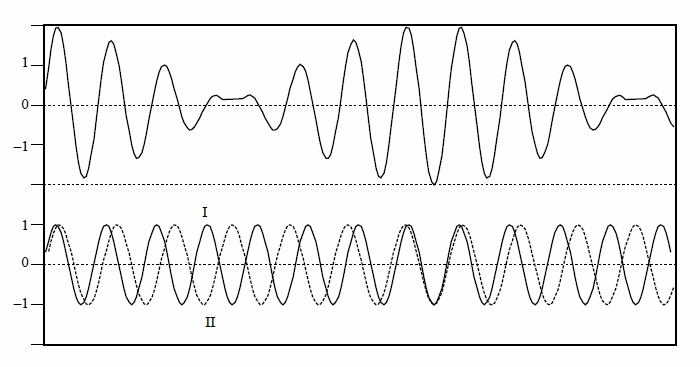
\includegraphics[width=8cm,height=6.4cm]{./02_Cap1/figures/fig_06_br.png}
\caption{\label{fig:bestserverarea}- Áreas Preditas de Melhor Servidor de Três Setores.}
\end{center}
\end{figure}

\section{\textbf{Classificação segundo o Método de Cálculo}}
\label{sec:Cap1Metodo}

O primeiro critério de classificação é a maneira pela qual os métodos de localização calculam a estimativa de posição do MS no plano. Para utilizar a geometria euclidiana, é necessário que as coordenadas geográficas dos setores de referência e do MS sejam representadas através uma projeção cartográfica retangular, ou seja, utilizando um sistema de coordenadas cartesianas. Os principais exemplos de sistemas de coordenadas retangulares utilizados em cartografia são o sistema UTM~(\textit{Universal Transverse Mercator})~\cite{Geocartografia}, que utiliza a projeção cartográfica transversa de Mercator, e o sistema MGRS~(\textit{Military Grid Reference System})~\cite{MGRS}.

\subsection{\underline{Identidade da Célula}}
\label{subsec:Cap1Cid}

No método de localização da identidade da célula~(CID - \textit{Cell Identity}), a posição do MS é assumida como sendo igual à da antena transmissora do setor melhor servidor. O método CID, embora seja de baixa complexidade e elevada disponibilidade, apresenta uma precisão muito dependente da densidade de setores na área de interesse~\cite{SPAWC2008}. Assim, o erro de localização pode variar de algumas centenas de metros em áreas urbanas até vários quilômetros em áreas rurais.

\subsection{\underline{Triangulação}}
\label{subsec:Cap1Triangulacao}

As técnicas de triangulação utilizam medidas de distâncias~(multi-lateração) ou ângulos~(multi-angulação) entre o MS e os setores de referência para estimar a localização do MS~\cite{LocationMethodsSurvey2007}.

Todos os métodos de triangulação presumem condições de propagação com linha de visada~(LOS - \textit{Line of Sight}) entre o MS e setores de referência. A propagação por múltiplos percursos e a presença de obstáculos entre o MS e os setores de referência podem corromper as medidas angulares, de tempo e de atenuação no percurso. Assim, a propagação sem linha de visada~(NLOS - \textit{Non Line of Sight}) é a principal fonte de erro para esses métodos. Como a propagação NLOS predomina em ambientes urbanos, a precisão dos métodos de triangulação pode ser seriamente comprometida nesses ambientes.

Além da propagação NLOS, outro fator que limita a precisão dos métodos de triangulação é a resolução finita das medidas realizadas na interface aérea e que são utilizadas no cálculo de posição: tempo, RSS e ângulo de chegada. A resolução da medida de RSS depende de especificações da interface rádio. Em redes GSM e WCDMA, por exemplo, os valores de RSS são reportados pelo MS em passos de $1$ dB~\cite{ETSI100911}~\cite{3GPP25133}. A resolução da medida angular depende da configuração dos conjuntos de antenas diretivas necessários para estimar o ângulo de chegada, bem como do diagrama de irradiação das antenas utilizadas no conjunto~\cite{Rappaport1997}.

\subsubsection{Multi-lateração Circular utilizando RTT}
Um valor de RTT pode ser convertido em uma estimativa de distância, através da equação~(\ref{eq:dist}). O lugar geométrico dos pontos que distam $\hat{d}_{i}$ da $i$-ésima célula de referência é um círculo de raio $\hat{d}_{i}$ centrado na posição desta célula. Esse círculo define o conjunto dos pontos no plano que contém a possível localização do MS, sendo denominado linha de posição (LOP - \textit{Line of Position}).

\begin{equation}
\label{eq:dist}
\hat{d}_{i}= \frac{c \cdot \textrm{T}_{s} \cdot \textrm{RTT}_{i}}{2}
\end{equation}

A medida de RTT tem resolução igual ao período de um símbolo. Porém, por razões de simplificação, utiliza-se a representação por meio de LOPs circulares, com raio igual ao raio interno no anel circular. Quanto menor o período de símbolo, menor é a largura do anel circular e mais este anel aproxima-se de um círculo. Assim, em sistemas banda larga, como o WCDMA, a utilização de LOPs circulares não introduz erro significativo~\cite{CidRttForcedHandover}.

\section{\textbf{Quadro Sinótico}}
\label{sec:Cap1Quadro}

A~\ref{tab:quadrosinotico} resume as principais características dos métodos de localização apresentados neste capítulo: o método de cálculo, a participação do MS no cálculo da posição, a quantidade mínima de setores requerida para calcular a posição do MS e os elementos adicionais necessários na rede de acesso rádio~(RAN - \textit{Radio Access Network}). A última coluna informa se o método depende de condições de propagação LOS entre o MS e as células de referência - ou os satélites, no caso do método AGPS - para não sofrer degradação da acurácia de localização.

Como a precisão de um método de localização é fortemente dependente das características específicas da rede onde o mesmo será utilizado - largura de banda, resolução temporal, densidade superficial de setores, ambiente de propagação, etc. - optou-se por não inserir na~\ref{tab:quadrosinotico} valores genéricos de precisão, como os fornecidos em~\cite{WlanLocationMethodsSurvey}.

\begin{table}[h]
\centering
\caption{\label{tab:quadrosinotico}- Quadro Sinótico dos Métodos de Localização.}
\vspace*{.1cm}
\begin{scriptsize}
\begin{tabular}{|c|c|c|c|c|c|}
\hline
\textbf{Sigla} & \textbf{Método de Cálculo} & \textbf{Participação} & \textbf{Quant. Mín.} & \textbf{Elem. adicionais} & \textbf{Requer}\\
& & \textbf{do MS} & \textbf{de Setores} & \textbf{na RAN} & \textbf{LOS ?}\\
\hline
AOA	& Triang. por multi-angulação & Baseado & 2	& Conj. de antenas & Sim \\
& & na Rede & & diretivas & \\
\hline
CID	& Identidade da célula	& Baseado & 1	& - & Não\\
& & na Rede & & & \\
\hline
EOTD	& Triang. por multi-lateração &	Assistido ou &	3	& LMUs & Sim \\
& hiperbólica & Baseado no MS & & & \\
\hline
AGPS	& Triang. por multi-lateração & Assistido & 3 & - & Sim \\
& circular & pelo MS & & & \\
\hline
CID+RTT	& Triang. por multi-lateração &	Baseado & 3	& - & Sim \\
& circular com RTT & na Rede & & & \\
\hline
CID+RSS	& Triang. por multi-lateração circular  &	Baseado & 3	& - & Sim \\
& com perda de propagação & na Rede & & & \\
\hline
AOA+RTT	& Híbrido	& Baseado & 1	&  Conj. de antenas & Sim \\
& & na Rede & & diretivas & \\
\hline
AOA+RSS	& Híbrido	& Baseado & 1	&  Conj. de antenas & Sim \\
& & na Rede & & diretivas& \\
\hline
AOA+TDOA	& Híbrido	& Assistido & 2	&  Conj. de antenas & Sim \\
& & pelo MS & & diretivas& \\
\hline
\end{tabular}
\end{scriptsize}
\vspace*{-.2cm}
\end{table}
\chapter{REVISÃO BIBLIOGRÁFICA}
\label{chapter:exemplo}
\section{\textbf{Sistemas Embarcados}}
\label{sec:SistemasEmbarcados}
\subsection{\textbf{Conceitos Preliminares}}
\label{subsec:sub01_Conceitos}

\subsection{\textbf{Definição de Sistemas Embarcados}}
\label{subsec:sub01_Definicao}
Um sistema embarcado pode ser definido, como um sistema computacional, interno a um dispositivo eletrônico, que executa, repetitivamente, uma única função, ou um pequeno conjunto de funções, de maneira que, frequentemente, a forma que estas tarefas são executadas não é percebida pelo seu usuário, assim como expõe \citeonline[p.~1]{Chatto2013}, mas sim os resultados da realização das mesmas. Já o termo “sistema embarcado” deriva do fato que estes sistemas são totalmente integrados e enclausurados pelos sistemas a que servem ou controlam, dessa forma, com este enclausuramento, tem-se como consequência que estes sistemas se tornam especializados em realizar tarefas específicas à operação do dispositivo que o contém, \cite[p.~554]{Springer2009}. Essa especialização é notada no software embarcado, também chamado de firmware, que se torna específico ao hardware utilizado, e o próprio hardware, que tem características que o diferem de um hardware de sistema de propósito geral. 

Com o objetivo de deixar mais claro o que essa falta de generalidade relacionada a funcionalidade de um sistema embarcado implica, \citeonline[p.~2]{Steve2003} complementa ao dizer que tais sistemas não são construídos de forma a serem programados pelo usuário final, não da forma que um sistema genérico possibilita, pois, o usuário final de um sistema embarcado não pode alterar a funcionalidade do sistema, seja adicionando, ou mesmo retirando, software. Observe, por exemplo, que um computador pessoal, um exemplo de sistema de propósito geral, pode funcionar como um processador de texto e, em um instante, começar a funcionar como um navegador web, observe ainda que, é permitido, ao usuário, adicionar diversas funcionalidades ao sistema, sem que o sistema tenha vindo configurado para execução da nova funcionalidade de fábrica. 

\subsection{\textbf{Características}}
\label{subsec:sub01_Caracteristicas}
Algumas características dos sistemas embarcados serão descritas a seguir, que é uma breve explanação sobre alguns pontos apresentados por \citeonline[p.~2-4]{Chatto2013}, importante notar que a exibição de todas estas características descritas não é obrigatória, porém, são muito comuns e importantes nestes sistemas, e, geralmente, alguma delas se sobressai, dependendo da finalidade do sistema em questão.

 A interação com o ambiente é uma característica presente na maioria dos sistemas embarcados, esta é feita por meio de sensores, que coletam dados do ambiente, e, ou, de atuadores, que atuam em alguns parâmetros do ambiente. Através da interação com o ambiente, os sistemas embarcados podem ser sistemas reativos, ou seja, possuir interação contínua e reagir a eventos do ambiente, onde o sistema pode, por exemplo, apresentar estados que transitam em resposta à ocorrência de eventos, ou reagir, com o objetivo de controlar algum tipo de variável do ambiente. Pode-se citar ainda, como uma característica, a mistura de componentes digitais e analógicos, que é inerente a interação com o ambiente. O ambiente, cuja natureza é predominantemente contínua. Portanto, frequentemente, a natureza digital dos computadores se mescla com a natureza analógica do ambiente para a implementação de um sistema embarcado.
 
A interface com o usuário, comumente, é mais simples que a encontrada em sistemas mais genéricos, composta por componentes que geralmente causam a ilusão ao usuário de falta de computação, como LEDs e botões.

A limitação do sistema, este que é restringido de diversos ângulos. Nota-se que, um sistema embarcado, pela sua própria natureza limitada, possui limitações de performance e de consumo de energia, que influenciam na escolha do dispositivo alvo. Como exemplo, o volume físico é uma limitação de projeto muito comum, dentre tantas outras limitações específicas de cada projeto, com sua relevância intrínseca ao projeto, como robustez a variação de temperatura, resistência a radiação, ou vibração mecânica. De fato, nenhum sistema é de todo livre de restrições, porém, nos sistemas embarcados, essas restrições são muito mais evidentes e são, em certos casos, consequência de requisitos do sistema.

A confiabilidade do sistema, já que, como um sistema embarcado tem a capacidade de funcionar autonomamente, estes são empregados em diversas atividades de natureza crítica, o que exige, frequentemente, disponibilidade e manutenibilidade do sistema e também segurança da informação processada pelo sistema. 

Relacionado à confiabilidade, está também a característica de processamento em tempo real, que se refere a exigência de resposta em um tempo fixo e finito de tempo de uma requisição. O não cumprimento desta exigência pode levar a consequências catastróficas em sistemas de tempo real. 

\subsection{\textbf{Elementos de um Sistema Embarcado}}
\label{subsec:sub01_Elementos}
Um sistema embarcado, geralmente, é um sistema microprocessado, isto significa que o mesmo, geralmente, se utiliza de uma unidade central para o processamento, o processador. Este processador pode ser implementado através de dispositivos de hardware programável, como um FPGA, ou se utilizar de um processador dedicado disponível no mercado, ou ainda, caso não se utilize um processador formal, um sistema embarcado poderia ser ainda implementado com a utilização de circuitos lógicos digitais, sem perca de sua condição de sistema embarcado. Porém, essas abordagens são geralmente mais complexas, e exigem um tempo de implementação maior do que o gasto quando um dispositivo com um processador pronto, que atende os requisitos do projeto, está disponível. Com esta visão, os microcontroladores aparentam ser grandes aliados dos sistemas embarcados.

\paragraph{\textbf{Microcontrolador -}}
Um microcontrolador, segundo \citeonline{Steve2003}, é um dispositivo que é autocontido e possui processador, memória e periféricos em um mesmo chip, o que, para projetistas de sistemas embarcados é de grande ajuda, já que a utilização destes elementos no sistema é feita através de software, poupando o projetista de futuros e eventuais complicações de interface e de compatibilidade. Caso se utilizasse um microprocessador ao invés de um microcontrolador, elementos externos deveriam ser adicionados para prover as funcionalidades fornecidas pelos periféricos e memória, porém, quando baseados em processadores dedicados, geralmente, os sistemas possuem maior performance computacional, em relação a sistemas baseados em microcontrolador, isto é devido ao hardware dedicado e otimizado para processamento, logo, o projetista deverá analisar se o esforço de implementação compensará o ganho computacional ao decidir a abordagem que deve seguir.
Na escolha de um microcontrolador, destacam-se alguns fatores importantes, \cite[p.8]{Chatto2013}, apresentados a seguir: 
\begin{itemize}
    \item Velocidade do microcontrolador:
    deve ser suficiente para o processamento requerido.
    \item Tamanho e encapsulamento do chip:
    pode interferir no tamanho do dispositivo final. 
    \item Espaço de memória:
    deve ser suficiente para armazenar a memória do sistema.
    \item Custo unitário do chip:
    não deve ser proibitivo para o custo do sistema.
    \item Recursos da plataforma de desenvolvimento:
    recursos podem ajudar no desenvolvimento do sistema, como por exemplo o recurso de debugging.
    \item Disponibilidade do chip no mercado:
    em um produto comercial pode implicar em maiores custos para manutenção e custos de produção.
\end{itemize}

Pode-se citar também como fator importante na escolha de um microcontrolador, a questão dos periféricos encontrados no chip, estes devem englobar os periféricos necessários para a implementação do sistema, ou, pelo menos que os periféricos faltantes possam ter sua funcionalidade implementada de uma outra maneira.

\paragraph{\textbf{Periféricos do Microcontrolador -}}
Um sistema embarcado, com sua característica de comunicação com o mundo exterior, necessita de periféricos. Os periféricos internos ao chip do microcontrolador são recursos implementados em hardware que podem ser utilizados por meio do software dentro do microcontrolador. Por exemplo, existem periféricos relacionados a comunicação, levantamento de interrupções (possibilitando tratamento de eventos esporádicos no sistema), temporização, contagem de eventos, leitura de dados analógicos, modulação de largura de pulso (possibilitando a geração de um sinal analógico), dentre outros periféricos mais específicos, internos ao chip do microcontrolador, evitando a implementação destes em hardware ou software. Periféricos podem ser adicionados a um sistema embarcado sem que sejam internos ao microcontrolador, a seguir, a fim de descrever alguns dos periféricos internos ao microntrolador, segue-se algumas informações sobre alguns deles.
\begin{itemize}
    \item Conversor analógico digital:
    Este periférico, tem a funcionalidade de interpretar valores analógicos de tensão e então convertê-los para valores digitais, assim, o processador poderá utilizar o dado medido para a aplicação no sistema. Com o grande número de sensores existentes, diversas grandezas, como temperatura ou pressão, podem ser convertidas para sinais de tensão e serem utilizadas pelo sistema por meio da utilização deste periférico.
    \item Timer:
    Um temporizador em hardware, de forma que seu funcionamento é independentemente da execução do software, o que permite maior robustez na medição de tempo. Um timer possui um tamanho máximo de contagem, e possui também registradores que armazenam o valor atual desta contagem. Quando o valor máximo de contagem for estourado, o timer pode gerar uma interrupção, produzindo uma rotina de tratamento de interrupção de estouro de timer. Uma aplicação de uso de um timer poderia ser a execução de rotinas periódicas. 
    \item Comunicação (USART, MSSP):
    A comunicação é importante pois permite a utilização de mais elementos no sistema atuando em conjunto, de fato, diversos elementos, como sensores, memórias ou displays se utilizam de uma interface de comunicação.  Quanto aos periféricos relacionados, eles existem para diferentes interfaces de comunicação, como SPI, I2C e RS232, por exemplo, que serão descritas mais adiante no texto. Para fim de exemplificação, em alguns microcontroladores PIC, existe um módulo de comunicação serial síncrona que suporta SPI e I2C (módulo MSSP) e um módulo de comunicação serial assíncrona que suporta RS-232 e RS-485 (módulo USART), \cite{pic18:DS39500A}. 
    \item PWM/Capture/Compare:
    Este periférico agrupa três possíveis funcionalidades do módulo, que são associadas a módulos de timer e um pino específico do microcontrolador. Em modo Compare, um valor determinado, escrito nos registradores deste módulo, é constantemente comparado com o valor de contagem do timer associado, quando o valor é atingido, ou seja, um tempo determinado se passa, o pino altera de nível lógico ou vai para um nível lógico definido, assim pode-se utilizar este recurso para a geração de um sinal. No modo Capture, algo parecido com o inverso do modo Compare é feito, neste modo, quando uma alteração no estado do pino associado ocorre, o valor da contagem do timer é capturado, assim, se pode medir o tempo entre os eventos no pino. Já o modo PWM permite que um sinal periódico possa ser gerado, através do pino associado, com tempos em nível alto e baixo que respeitam o ciclo de trabalho definido, ou duty cycle, este parâmetro define o tempo que o sinal passará em alto com relação ao período do sinal periódico, assim, por exemplo, um duty cycle de 30\% indica que o sinal passará 30\% do período em nível alto. O PWM é uma sigla que vem de Pulse Width Modulation, ou seja, modulação de largura de pulso, pois gera um trem de pulsos com largura controlada, este periférico pode ser usado como sinal para comandar motores de corrente contínua por exemplo.\cite{pic18:DS39500A}. 
\end{itemize}

Além destes periféricos, um periférico interessante é o de interrupção externa, este possibilita o levantamento de uma interrupção no sistema, que, por sua vez, leva a execução de uma rotina de interrupção. A interrupção, para este periférico, é levantada quando uma mudança de estado de um pino específico acontece, assim, através desta funcionalidade, diversos eventos podem executar uma rotina de tratamento. Interessante dizer que essa interrupção pode ser gerada a qualquer momento, desde que esteja habilitada, bastando para isso que o evento em questão altere o estado do pino específico do microcontrolador.

% inserir demais capítulos aqui
% -----------------------------
% -----------------------------
% -----------------------------
% -----------------------------





\pagebreak
\addcontentsline{toc}{chapter}{\hspace{1.7cm}\bfseries CONCLUSÃO}
\noindent\textbf{CONCLUSÃO}
$\!$\\

Aqui entra sua conclusão!!

\pagebreak
\addcontentsline{toc}{chapter}{\hspace{1.7cm}\bfseries REFERÊNCIAS}
\def\bibname{REFERÊNCIAS}




% abaixo segue a chamada para o arquivo [.BIB]. Utilizei o programa JABREF para montar o arquivo com minhas referências.
\bibliography{dissertacao}



%felipe% \printindex    %Removi o índice remissivo para a versão oficial do trabalho.


\end{document}